\documentclass[11pt]{article}
\usepackage[margin=1in]{geometry}
\usepackage{amsmath,amssymb,amsthm}
\usepackage{graphicx}
\usepackage{xcolor}
\usepackage[colorlinks=true,linkcolor=blue,citecolor=blue,urlcolor=blue]{hyperref}

\newtheorem{prop}{Proposition}
\newcommand{\dd}{\mathrm{d}}
\newcommand{\E}{\mathbb{E}}

\title{\textbf{Step 1: the growth exponent $\alpha$}\\[2pt]
\large from recurrent churn to hegemonic lock-in}
\author{M.\ Heltberg}
\date{Stepwise-progression note, June 2026}

\begin{document}
\maketitle

\noindent\emph{Folder \texttt{stepwise\_progression/}. Code:
\texttt{step1\_alpha.py}. Builds on \texttt{ANALYSIS\_step0.tex}.}

\begin{abstract}
We generalise the growth drift to $\dd S_i=\gamma_i R\,S_i^{\alpha}\,\dd t$
($+$ demographic noise) and ask how the exponent $\alpha$ controls the rise and
fall of dominant states. The answer is governed by the \emph{relative} dynamics:
the log-ratio of any two states has a growth-drift $\propto
S_i^{\alpha-1}-S_j^{\alpha-1}$, whose sign flips at $\alpha=1$. For $\alpha<1$ a
lead is \emph{eroded} (sub-linear returns let laggards catch up $\Rightarrow$
recurrent turnover, the Step-0 churn); at $\alpha=1$ the log-ratio is driftless
(marginal); for $\alpha>1$ a lead is \emph{amplified} (super-linear returns
$\Rightarrow$ a durable hegemon). Simulations confirm the mean leader lifetime
rising from $\sim4$ at $\alpha=0$ to $\sim100$ (half the run) at $\alpha=2$, with
the transition at $\alpha=1$. A second, distinct threshold $\alpha=\tfrac12$
(drift vs.\ noise of a single state) governs absolute, not relative, stability.
\end{abstract}

% ====================================================================
\section{Model}

\begin{equation}
R=\max\!\Big(1-\tfrac1K\textstyle\sum_jS_j,0\Big),\qquad
\dd S_i=\gamma_i R\,S_i^{\alpha}\,\dd t+\sigma\sqrt{S_i}\,\dd W_i,
\label{eq:model}
\end{equation}
with $\gamma_i$ a positive-mean OU process (so growth is sustained and $\alpha$ is
isolated). $\alpha=0$ recovers the additive Step-0 model; $\alpha=1$ is
multiplicative growth. We keep the demographic noise $\sigma\sqrt{S_i}$ fixed and
vary only $\alpha$.

% ====================================================================
\section{Phenomenology}

The character of the dynamics changes smoothly with $\alpha$
(Fig.~\ref{fig:alpha}, $20$ seeds):
\begin{center}
\begin{tabular}{lrrrrrrrr}
$\alpha$ & 0 & 0.25 & 0.5 & 0.75 & 1.0 & 1.25 & 1.5 & 2.0\\
\hline
leadership changes & 67 & 50 & 50 & 54 & 47 & 33 & 33 & 14\\
mean leader lifetime & 3.8 & 5.3 & 6.4 & 8.1 & 10.9 & 21.9 & 41.8 & 99.2\\
\end{tabular}
\end{center}
Inequality is high (Gini $\approx0.85$, top share $\approx0.85$) at \emph{all}
$\alpha$: condensation onto a few states is the generic Step-0 effect of the
$\sqrt S$ noise. What $\alpha$ tunes is not the \emph{degree} of concentration but
its \emph{persistence} --- whether the condensate moves (churn) or sticks
(lock-in).

\begin{figure}[h]
\centering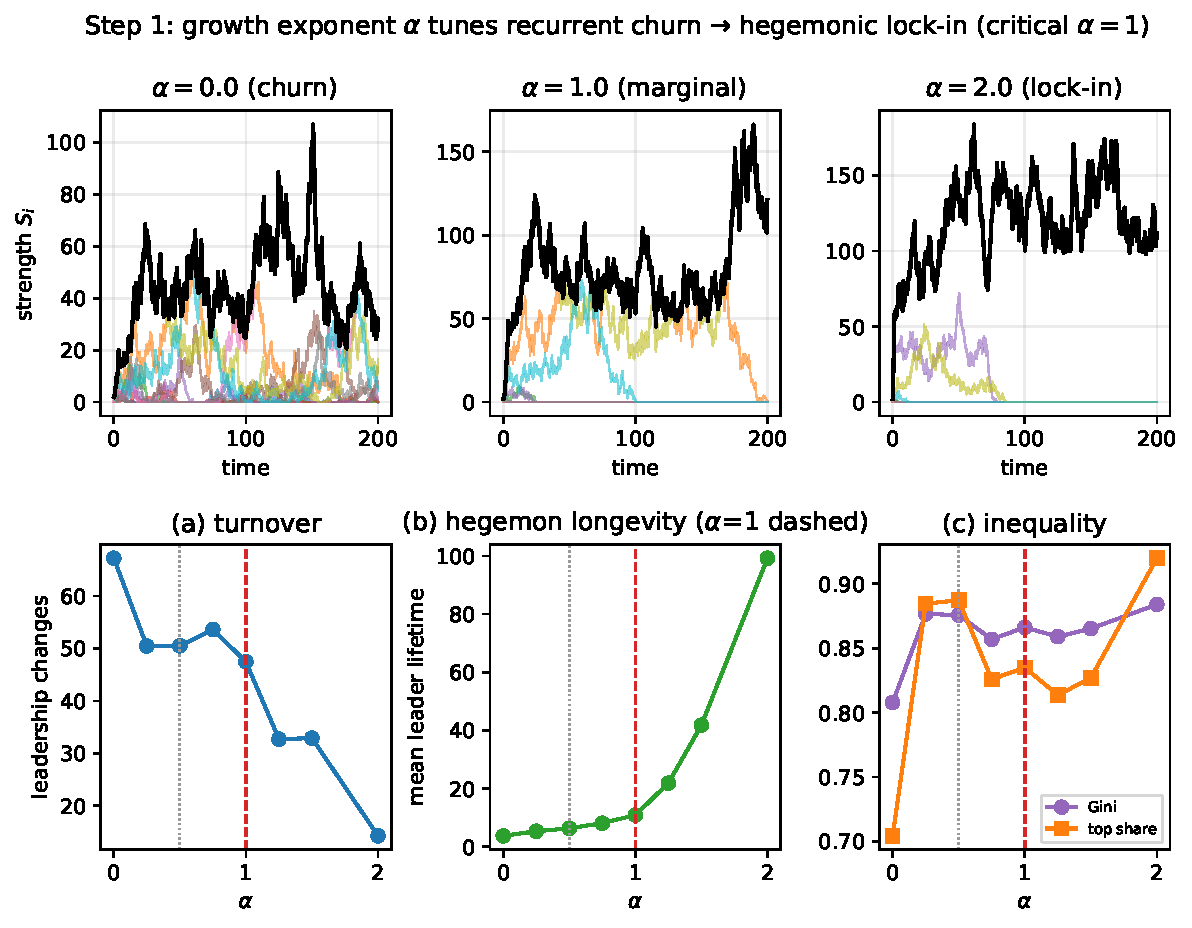
\includegraphics[width=\textwidth]{figs/step1_alpha.pdf}
\caption{Top: example trajectories (leader in black) at $\alpha=0$ (churn),
$1$ (marginal), $2$ (lock-in). Bottom: leadership changes (a), mean leader
lifetime (b), and inequality (c) vs $\alpha$; the dashed red line marks the
relative-lock-in transition $\alpha=1$, the dotted grey line the
absolute-stability threshold $\alpha=\tfrac12$.}
\label{fig:alpha}
\end{figure}

% ====================================================================
\section{The relative dynamics: critical $\alpha=1$}\label{sec:rel}

Leadership is a question about \emph{ratios} of strengths, so we study the
log-strength. By It\^o on \eqref{eq:model} with $f=\ln S$
($f'=1/S,\ f''=-1/S^2,\ (\dd S)^2=\sigma^2S\,\dd t$),
\begin{equation}
\dd\ln S_i=\Big[\gamma_i R\,S_i^{\alpha-1}-\frac{\sigma^2}{2S_i}\Big]\dd t
            +\sigma\,S_i^{-1/2}\,\dd W_i .
\label{eq:dlnS}
\end{equation}
For two states with a common rate $\gamma$, the log-ratio $u=\ln(S_i/S_j)$ obeys
\begin{equation}
\dd u=\underbrace{\gamma R\big(S_i^{\alpha-1}-S_j^{\alpha-1}\big)}_{\text{growth}}\dd t
      \;\underbrace{-\;\frac{\sigma^2}{2}\Big(\frac1{S_i}-\frac1{S_j}\Big)}_{\text{It\^o (subdominant)}}\dd t
      \;+\;\sigma\big(S_i^{-1/2}\dd W_i-S_j^{-1/2}\dd W_j\big).
\label{eq:du}
\end{equation}
The leading (growth) drift contains $g(S)=S^{\alpha-1}$, with
$g'(S)=(\alpha-1)S^{\alpha-2}$. Hence, taking $S_i>S_j$ (state $i$ ahead):
\begin{equation}
\operatorname{sign}\big(\text{growth drift of }u\big)
=\operatorname{sign}(\alpha-1).
\end{equation}
\begin{itemize}
\item $\boxed{\alpha<1}$ — \emph{diminishing returns}: $g$ decreasing, so the
  leader's per-capita growth $\gamma R S^{\alpha-1}$ is \emph{smaller} than the
  laggard's. The log-ratio mean-reverts toward $0$: leads erode, the laggard
  catches up, and the demographic noise then reshuffles the order — \textbf{recurrent
  churn} (this includes Step 0, $\alpha=0$).
\item $\boxed{\alpha=1}$ — \emph{constant returns}: $g\equiv1$, the growth drift
  of $u$ vanishes and $u$ is a (noise-driven) martingale — \textbf{marginal}.
  Turnover still occurs but only by diffusion of the ratio, so reigns lengthen.
\item $\boxed{\alpha>1}$ — \emph{increasing returns}: $g$ increasing, the leader
  grows faster \emph{per capita}; the log-ratio drift is positive and the lead is
  amplified — \textbf{hegemonic lock-in}.
\end{itemize}
The It\^o term $-\tfrac{\sigma^2}{2}(S_i^{-1}-S_j^{-1})>0$ for $S_i>S_j$ adds a
small leader-stabilising drift that vanishes as the states grow; it shifts the
balance slightly but does not change the $\alpha=1$ sign flip. The noise variance
$\sigma^2(S_i^{-1}+S_j^{-1})$ is dominated by the \emph{smaller} state, so
relative fluctuations are largest among small states — turnover happens while the
contenders are still small.

\paragraph{Equivalent deterministic picture (a bifurcation at $\alpha=1$).} Drop
the noise and let $\rho=S_i/S_j$. From \eqref{eq:model},
\begin{equation}
\frac{\dd}{\dd t}\ln\rho=\gamma R\,(S_i^{\alpha-1}-S_j^{\alpha-1})
=\gamma R\,S_j^{\alpha-1}\big(\rho^{\alpha-1}-1\big).
\end{equation}
The fixed point $\rho=1$ (equality) is \emph{stable} for $\alpha<1$ and
\emph{unstable} for $\alpha>1$: a pitchfork-like exchange of stability in relative
position. For $\alpha>1$ any initial lead runs away ($\rho\to\infty$); indeed the
bare ODE $\dot S=\gamma R S^\alpha$ has super-linear, finite-time-blow-up
character, capped here only by $R\downarrow0$ — the hegemon saturates at the
resource limit rather than diverging.

% ====================================================================
\section{The other threshold: $\alpha=\tfrac12$ (absolute stability)}

A \emph{single} state's drift-to-noise ratio is
\begin{equation}
\frac{\text{drift}}{\text{noise rate}}=\frac{\gamma R\,S^{\alpha}}{\sigma\sqrt S}
=\frac{\gamma R}{\sigma}\,S^{\alpha-1/2},
\end{equation}
which is scale-invariant at $\alpha=\tfrac12$. For $\alpha<\tfrac12$ a large state
is noise-dominated (its \emph{absolute} size is hard to maintain — relevant to
whether a state can climb from small values or is pushed toward $0$); for
$\alpha>\tfrac12$ size is self-reinforcing. This is a statement about absolute
sizes, \emph{not} about who leads, and it is why the visible turnover transition
sits at $\alpha=1$ (relative) while inequality is already high well below it.
Step 0's collapse argument ($\alpha=0<\tfrac12$, a driftless $\sqrt S$ Bessel
martingale absorbed at $0$) is the extreme case.

% ====================================================================
\section{How $\alpha$ changes the rise and collapse of nations}

\begin{itemize}
\item $\alpha<1$ (\emph{diminishing returns}). Leads erode; dominance is short
  and recurrent. Many states take turns on top; collapses are frequent and
  shallow. Mean reign $\sim$ a few time units. The natural ``balance-of-power''
  regime.
\item $\alpha=1$ (\emph{constant returns}). Marginal: the relative order is a
  martingale, so turnover is slow (reigns $\sim$ tens of units) and driven purely
  by fluctuations — no mechanism either erodes or entrenches a lead.
\item $\alpha>1$ (\emph{increasing returns}). A single hegemon locks in and
  persists for most of the observation window; collapses become \emph{rare} but,
  when a large fluctuation finally unseats the giant, \emph{deep} — long, dramatic
  hegemonic cycles rather than rapid churn.
\end{itemize}
Empirically (Fig.~\ref{fig:alpha}b) the mean reign grows by $\sim\!25\times$ across
$0\le\alpha\le2$, with the knee at $\alpha=1$, exactly as \S\ref{sec:rel} predicts.

% ====================================================================
\section{Caveat and outlook}

The \texttt{max(S,0)} clamp again injects a little mass under the $\sqrt S$ noise
(see Step 0); use a positivity-preserving CIR scheme for long-time quantitative
work. The exponent $\alpha$ is the cleanest single knob for the rise-and-fall
character and is a natural control parameter to carry into the later steps: a
\emph{conflict} mechanism (Step 2) that transfers strength to the winner is itself
an effective increasing-returns ($\alpha>1$-like) force, so we expect war to push
an otherwise churning ($\alpha<1$) world toward lock-in --- a competition between
the growth exponent and the conflict rule that the next step will make explicit.

\end{document}
